% !TeX encoding = ISO-8859-1
% Bachelor Thesis/Master Thesis Template
% based on Disseration Template by J�rn Malzahn:
% Last update: 2015/02/19 cr
% This template has been designed to be compliant with the requirements of the VDI Verlag-
% See VDIVerlag-Hinweise-31_03_2013.pdf for details. The basic principle of these requirements is: you submit a compliant A4 print and they will guarantee a high quality A5 book.
%
%
% NOTE: The template is still under developement.


\documentclass[12pt,a4paper,twoside,headsepline,captions=tableheading,toc=bibliography,openany]{scrbook}

%% For a draft version of your thesis use this line.
%\documentclass[draft,12pt,a4paper,twoside,headsepline,captions=tableheading,toc=bibliography,openany]{scrbook}
%% It uses the draft switch, which will not include the graphics in your output document. Instead it draws bounding boxes for each figure and highlights overfull boxes, and highlights exceeding margins. This is particularly usefull to hunt down overfull boxes.

% useful scripts including if/then/else
\usepackage{etoolbox}

% set language to english, compile two times after changing
\newtoggle{lang_eng}
\settoggle{lang_eng}{false} % true: english, false: german

%Self-defined hyphenations
% !TeX encoding = ISO-8859-1
% Just continue this space separated list
\hyphenation{Tech-ni-sche Uni-ver-si-t�t Dort-mund}

% additional packages
%% The following commented packages are included in the Beamer style template
%%\usepackage{pgfcomp-version-0-65}
%%\usepackage{xcolor}
%%\usepackage{graphicx}
%%\usepackage{pgfplots}
%%\usepackage{epstopdf}
%%\usepackage{changepage}
%%\usepackage{etoolbox}
%%\usepackage{helvet}


\usepackage[utf8]{inputenc}
\usepackage[\iftoggle{lang_eng}{english}{ngerman}]{babel}

\usepackage[justification=centering]{caption} % Justification: center captions by default
\captionsetup{textfont=scriptsize, font=scriptsize,labelfont=scriptsize}
\captionsetup[subfigure]{skip=7pt} % vertical spacing between figure and subfigure caption
\captionsetup{aboveskip=3pt} % vertical spacing between subfigure caption and figure caption (\baselineskip + aboveskip)
\captionsetup{belowskip=3pt} % vertical spacing between subfigure caption and figure caption (\baselineskip + aboveskip)

%% REMOVE LABELS a), b), ... Put this into figure environments for local settings
%\captionsetup[figure]{labelformat=empty}
%\captionsetup[subfigure]{labelformat=empty} 
%\captionsetup[table]{labelformat=empty}
%% You can easily hide labels by using \caption*{} instead of \caption{}

%\captionsetup[subfigure]{labelformat=empty}
%\setbeamerfont{caption}{size=\tiny}

\usepackage{hyperref}

\usepackage{listings} % Für Code

\usepackage[locale=DE]{siunitx} % Für Einheiten


\usepackage{mathtools,amssymb,amsmath}

\usepackage{pgfpages} % required for showing notes on the second screen

\usepackage{algorithm} % selber eingebunden
\usepackage[noend]{algpseudocode} % Alternative Algorithmenumgebung
\newcommand*\Let[2]{\State #1 $\gets$ #2}

\usepackage{booktabs}

\usepackage{subcaption}

% Textbox
\usepackage{grid-system}


\usepackage{ifplatform}






% Path to the graphics/figures
\graphicspath{{./Abbildungen/}} 

% Disable automatic parindent (Einr�ckung nach jedem Abschnitt ausschalten)
\setlength{\parindent}{0cm}

%% To keep the overview, create a commented structure or obtain a ready to print version of your work:
% Variant I: Summary only: 
%\includecomment{summary} %Build latex code within summary environment
%\excludecomment{content} %Do not build latex code within the content envrionment
%% Variante II: Nur Inhalt:
%\excludecomment{summary} %Do not build latex code within the summary environment
%\includecomment{content} %Build latex code within content envrionment
%% Variante III: Summary + Inhalt:
\includecomment{summary} %Build latex code within summary environment
\includecomment{content} %Build latex code within content envrionment


% ##########################################################################
% BODY
% ##########################################################################
\begin{document}
%% Uncomment the following three lines to display the page layout. In that case also uncomment line 10 in packages.tex!
%\printinunitsof{cm}
%\currentpage
%\pagedesign

% ##########################################################################
% PREFACE AND INDEXES
% ##########################################################################
% Self-defined environments 
% !TeX encoding = windows-1252
\theoremstyle{myTheoremStyle}

\newtheorem{acknowledgement}{\iftoggle{lang_eng}{Acknowledgement}{Danksagung}}
%\newtheorem{algorithm}{\iftoggle{lang_eng}{Algorithm}{Algorithmus}}[section] % Use package algorithm instead, see packages.tex
\newtheorem{assumption}{\iftoggle{lang_eng}{Assumption}{Annahme}}[section]
\newtheorem{assumptions}{\iftoggle{lang_eng}{Assumptions}{Annahmen}}[section]
\newtheorem{axiom}{Axiom}[section]
\newtheorem{case}{\iftoggle{lang_eng}{Case}{Fall}}[section]
\newtheorem{claim}{\iftoggle{lang_eng}{Claim}{Forderung}}[section]
\newtheorem{conclusion}{\iftoggle{lang_eng}{Conclusion}{Schlussfolgerung}}[section]
\newtheorem{condition}{\iftoggle{lang_eng}{Condition}{Bedingung}}[section]
\newtheorem{conjecture}{\iftoggle{lang_eng}{Conjecture}{Vermutung}}[section]
\newtheorem{convention}{\iftoggle{lang_eng}{Convention}{Konvention}}[section]
\newtheorem{corollary}{\iftoggle{lang_eng}{Corollary}{Korollar}}[section]
\newtheorem{criterion}{\iftoggle{lang_eng}{Criterion}{Kriterium}}[section]
\newtheorem{definition}{Definition}[section]
\newtheorem{example}{\iftoggle{lang_eng}{Example}{Beispiel}}[section]
\newtheorem{exercise}{\iftoggle{lang_eng}{Exercise}{Aufgabe}}[section]
\newtheorem{lemma}{Lemma}[section]
\newtheorem{notation}{\iftoggle{lang_eng}{Notation}{Bezeichnung}}[section]
\newtheorem{problem}{Problem}[section]
\newtheorem{proposition}{\iftoggle{lang_eng}{Proposition}{Satz}}[section]
\newtheorem{remark}{\iftoggle{lang_eng}{Remark}{Bemerkung}}[section]
\newtheorem{solution}{\iftoggle{lang_eng}{Solution}{L�sung}}[section]
\newtheorem{theorem}{Theorem}[section]
\numberwithin{equation}{section}
%-----------------------------------------------------------
% Page numbering for title, abstract, dedication and acknowledgements
% Table of contents has roman page numbering. See VDIVerlag-Hinweise-31_03_2013.pdf for details.
\pagenumbering{roman}
\pagestyle{empty} 

%% Title page
\iftoggle{lang_eng}
	{\makeatletter  % Do not delete this line



\title{
\begin{table}[t]
	\begin{tabular}{p{0.775\columnwidth} r} % 0.775 was 0.85 -> needs a proper fix!
	%  \includegraphics[width=9cm]{tudo} & \includegraphics[width=2.5cm]{rst} \\
		
\includegraphics[width=9cm]{tud_logo_rgb} & 
\includegraphics[width=2.5cm]{rst_rgb}
	\end{tabular}
\end{table}
\LARGE Title of my thesis\\ 
\vspace{0.5cm}
\large{Subtitle (optional) }\\
\vspace{2cm}
{\normalfont\large{{\textbf{Master Thesis / Bachelor Thesis}}}\\ 
\vspace{1cm}
\normalfont{submitted to}\\
\vspace{1cm}
\normalfont{Institute of Control Theory and Systems Engineering}\\
\vspace{0.5cm} 
%\normalfont{der}\\
\normalfont{Faculty of  Electrical Engineering and Information Technology}\\ 
%\normalfont{der}\\
\vspace{0.5cm} 
\normalfont{Technische Universit�t Dortmund}\\
\vspace{1cm}
\normalfont{by}\\ 
\vspace{-1cm}
}}
\author{\normalsize{\normalfont{ Jane Doe }}\\ 
\normalsize{\normalfont{Birthplace, Native country}}}
\date{\vspace{2cm}
\raggedright{
\normalsize{\normalfont{Date of Submission: \today }\\ 
\vspace{0.5cm}
\normalfont{\textit{Responsible Professor}: }\\
\normalfont{Univ.-Prof. Dr.-Ing. Prof. h.c. Dr. h.c. Torsten Bertram}\\
\vspace{0.25cm}
\normalfont{\textit{Academic Supervisors}:}\\ 
\normalfont{Dipl.-Ing. Max Mustermann}\\
\normalfont{Dipl.-Ing. Lisa M�ller}\\
}}
}

\makeatother  % Do not delete this line
}
	{\makeatletter  % Do not delete this line



\title{
\begin{table}[t]
	\begin{tabular}{p{0.775\columnwidth} r} % 0.775 was 0.85 -> needs a proper fix!
	%  \includegraphics[width=9cm]{tudo} & \includegraphics[width=2.5cm]{rst} \\
		
\includegraphics[width=9cm]{tud_logo_rgb} & 
\includegraphics[width=2.5cm]{rst_rgb}
	\end{tabular}
\end{table}
\LARGE Titel meiner Abschlussarbeit\\ 
\vspace{0.5cm}
\large{Untertitel (optional) }\\
\vspace{2cm}
{\normalfont\large{{\textbf{Masterarbeit / Bachelorarbeit}}}\\ 
\vspace{1cm}
\normalfont{eingereicht am}\\
\vspace{1cm}
\normalfont{Lehrstuhl f�r Regelungssystemtechnik}\\
\vspace{0.5cm} 
%\normalfont{der}\\
\normalfont{Fakult�t f�r Elektrotechnik und Informationstechnik}\\ 
%\normalfont{der}\\
\vspace{0.5cm} 
\normalfont{Technische Universit�t Dortmund}\\
\vspace{1cm}
\normalfont{von}\\ 
\vspace{-1cm}
}}
\author{\normalsize{\normalfont{ Jane Doe }}\\ 
\normalsize{\normalfont{Geburtsort, Geburtsland}}}
\date{\vspace{2cm}
\raggedright{
\normalsize{\normalfont{Abgabedatum: \today }\\ 
\vspace{0.5cm}
\normalfont{\textit{Verantwortlicher Hochschullehrer}: }\\
\normalfont{Univ.-Prof. Dr.-Ing. Prof. h.c. Dr. h.c. Torsten Bertram}\\
\vspace{0.25cm}
\normalfont{\textit{Wissenschaftliche Betreuer}:}\\ 
\normalfont{Dipl.-Ing. Max Mustermann}\\
\normalfont{Dipl.-Ing. Lisa M�ller}\\
}}
}

\makeatother  % Do not delete this line
}
\maketitle

%% dedication
% !TeX encoding = ISO-8859-1
\thispagestyle{empty}
\vspace*{\fill}
\begin{center}
\begin{quote}
"\textit{Das ist die Widmung (optional)}"
\end{quote}
\end{center}
\vspace*{\fill}


\cleardoublepage % force next part to start on the right page

%% acknowledgement
% !TeX encoding = ISO-8859-1
\chapter*{\iftoggle{lang_eng}{Acknowledgement}{Danksagung}}
Das ist die Danksagung (optional)


\cleardoublepage % force next part to start on the right page

%% abstract
% !TeX encoding = ISO-8859-1
\chapter*{\iftoggle{lang_eng}{Abstract}{Kurzfassung}}
Das ist die Kurzfassung. Hier sollte klar werden womit sich die Arbeit besch�ftigt und die wichtigsten Aussagen sollen zusammengefasst werden. Richtwert is eine halbe Seite.

\cleardoublepage % force next part to start on the right page
  

% ##########################################################################
% MAIN CONTENTS
% ##########################################################################
% There is no list of figrues and list of tables in the template. See VDIVerlag-Hinweise-31_03_2013.pdf for details.
\setcounter{page}{1}
\pagestyle{headings} 
\tableofcontents
\newpage

%% nomenclature
% !TeX encoding = ISO-8859-1
%%%%%%%%%%%%%%%%%%%%%%%%%%%%%%%% Nomenclature %%%%%%%%%%%%%%%%%%%%%%%%%%%%%%%%%%%
%See: http://blog.stefan-macke.com/2006/05/03/abkurzungsverzeichnis-mit-latex/

% Page style
\markboth{\nomname}{\nomname}% maybe with \MakeUppercase
\iftoggle{lang_eng}{}{\renewcommand{\nomname}{Nomenklatur}} % use german name


\printnomenclature[4cm] % There is a bug TeXnicCenter version 2.0 Beta 1. As soon as this line is added to the document the structure pane indicates a missing paragraph. Nevertheless the nomenclature package works correctly. 

%% General variables
\nomenclature{$\mathbf{x}(t)$}{Zustandsvektor zum Zeitpunkt $t$}%
\nomenclature{$u(t)$}{Eingangssignal zum Zeitpunkt $t$}%
\nomenclature{$t$}{Zeit}
\nomenclature{$x,y,z$}{Spatial coordinates}

%% Abk�rzungen
\nomenclature[A]{Abrev.}{Abbreviation}
\nomenclature[A]{KF}{\textbf{K}alman \textbf{F}ilter}

\nomenclature[B]{$\alpha$}{Griechischer Buchstabe}


\cleardoublepage % fixes confused odd/even page order

%% Page numbering in the main part
\pagenumbering{arabic}
\pagestyle{headings} 

% #######################################################
% !TeX encoding = ISO-8859-1
\chapter{Aufbau der Arbeit}
\label{aufbau}

Im Vordergrund der Arbeit sollte die Dokumentation der eigenen
Arbeiten und Ergebnisse stehen, wobei eine Analyse, Interpretation
und Bewertung der angewendeten Methodik und der erzielten
Ergebnisse von zentraler Bedeutung sind.

Zu Beginn einer jeden wissenschaftlichen Arbeit sollte das
Literaturstudium stehen. Dieses sollte �ber den gesamten Zeitraum
der Arbeit andauern. Hierzu sind neben der Universit�tsbibliothek
auch weitere �ffentliche Datenquellen heranzuziehen. Insbesondere
eignet sich auch das Internet zur Recherche, dabei ist allerdings
auch die Herkunft der Quellen zu ber�cksichtigen. Auf Seiten wie
beispielsweise:

\emph{http://scholar.google.de/}

\emph{http://www.sciencedirect.com/}

\emph{http://citeseer.comp.nus.edu.sg/cs}

\emph{http://ieeexplore.ieee.org/search/advsearch.jsp}

\emph{http://www.springerlink.com/}

lassen sich zumeist relevante und auch vertrauensw�rdige
Ver�ffentlichungen finden. Im Vordergrund steht dabei eine
kritische Bewertung der aktuellen Literatur. In der Arbeit sind
nur Quellen auszuwerten, die f�r die zu bearbeitende Aufgabe
relevant sind. Aus der Analyse der Literatur und der Analyse der
aktuellen praktischen Erfordernisse der Aufgabenstellung ergibt
sich die tats�chliche Problemstellung. Diese ist zu Beginn der
Arbeit darzustellen. Bei der Erarbeitung der L�sung der Aufgaben
und der Darstellung der Ergebnisse kommen die Vorgehensweisen, die
Sie sich im Laufe des Studiums angeeignet haben zum Einsatz.
W�hrend der Bearbeitung der Thematik ist besonders darauf zu
achten, dass die erhobenen Daten so objektiv wie m�glich erfasst
und durch ausreichende Untersuchungen gest�tzt werden. Die
Beschreibung hat so zu erfolgen, dass die Nachvollziehbarkeit
gegeben ist. Die Beschreibung schlie�t dabei eine Diskussion und
Interpretation ein. Der Umfang der schriftlichen Ausarbeitung
liegt f�r eine Bachelorarbeit bei in etwa 30 Seiten und f�r eine
Masterarbeit bei in etwa 60 Seiten. Ein ausf�hrlich
beschriebener Leitfaden zur Gestaltung der schriftlichen
Ausarbeitung sowie zur Angabe der verwendeten Quellen ist
beispielsweise in \textcite{Leit1} zu finden.

\section{Hinweise zum Titelblatt}
\label{hinweise:titelblatt}

Das Titelblatt gibt Auskunft �ber das Thema der Arbeit, den
Lehrstuhl, Datum der Abgabe sowie den Namen der
Kandidatin bzw. des Kandidaten. Die entsprechenden Felder sind anzupassen.

\section{Hinweise zur Kurzfassung}
\label{hinweise:kurzfassung}

Die Kurzfassung (Abstract) sollte einen kurzen �berblick �ber das
Ziel und den Inhalt der Arbeit geben. Der Umfang sollte in etwa
bei einer halben DIN-A4-Seite liegen.

\section{Hinweise zum Inhaltsverzeichnis}
\label{hinweise:inhaltsverzeichnis}

Das Inhaltsverzeichnis stellt den logischen Aufbau der Arbeit dar.
Die Gliederung hilft die Struktur der Arbeit zu verdeutlichen. Die
Gliederungstiefe sollte angemessen gew�hlt werden und im
Normalfall nicht mehr als zwei Untergliederungsstufen pro Kapitel
enthalten.

\section{Hinweise zur Nomenklatur}
\label{hinweise:nomenklatur}

Die Nomenklatur sollte alle Bezeichnungen der in der Arbeit
verwendeten Symbole, Variablen, Abk�rzungen und deren Erkl�rungen
enthalten. Um die Eintr�ge der Symbole komfortabler zu generieren,
kann das nomencl-Paket verwendet werden: \\
\emph{http://www.ctan.org/tex-archive/macros/latex/contrib/nomencl/}.
Die tex-Dateien werden durch
\textit{makenomenclature} nach \textit{nomencl}-Aufrufen gescannt.
Es entsteht eine Datei \textit{struktur.nlo}, welche die Eintr�ge enth�lt.
Die Eintr�ge werden mit \textit{makeindex.exe} verarbeitet und dann mit
\textit{printnomenclature} ins das Latex-Dokument eingef�gt.
Ein Beispiel ist Abschnitt~\ref{hinweise:gleichungen} zu entnehmen.

\subsection{Vorgehensweise zur Einrichtung des Nomenklatur-Compilers}

\subsubsection{TeXstudio}
\textit{Optionen} $\rightarrow$ \textit{TeXstudio konfigurieren ...} $\rightarrow$ \textit{Befehle} $\rightarrow$ Zeile \textit{Makeindex}:
\begin{quotation}
makeindex.exe \%.nlo -s nomencl.ist -o \%.nls 
\end{quotation}

\noindent Einstellungen testen: F11 oder \textit{Tools} $\rightarrow$ \textit{Index}. \\
Falls erfolgreich, PDF neu erstellen. \textit{Makeindex} muss jedes Mal erneut aufgerufen werden, falls die Nomenklatur ge�ndert wurde. \\
Siehe \textit{nomenclature.tex} f�r Beispiele zur Erstellung der Nomenklatur.

\subsubsection{Bugs}

Sollten die Abst�nde in der Nomenklatur nicht korrekt sein und somit die Beschreibungen der Symbole nicht angezeigt werden, kann es helfen den Einzug der Beschreibung manuell zu setzen. Dazu wird in der Datei \textit{nomenclature.tex} die Zeile mit dem Befehl \textit{\textbackslash printnomenclature} erweitert zu \textit{\textbackslash printnomenclature[<Einzug>]}. \textit{<Einzug>} ist die Einzuggr��e der Beschreibung. Ein Einzug von 4cm entspricht in etwa dem Standardeinzug in dieser Beispiel Nomenklatur (Die Einzuggr��e ist standardm��ig gleich \textit{\textbackslash nomlabelwidth}. F�r weitere Informationen siehe Dokumentation des \textit{nomencl} Pakets). 


\section{Hinweise zur Struktur}
\label{hinweise:struktur}

Allgemeine Aussagen zu Inhalt und Struktur sind schwer m�glich. Die nachfolgenden Hinweise k�nnen im Einzelfall nicht zutreffend sein. Im Zweifel ist dar�ber mit dem Betreuer der Arbeit zu diskutieren.
Der Inhalt der schriftlichen Ausarbeitung kann beispielsweise wie
folgt gegliedert werden:

\begin{itemize}
	\item Einleitung
	\item Theoretischer Teil
	\item Eigene Untersuchungen
	\item Experimentelle / simulative Ergebnisse
	\item Zusammenfassung / Ausblick
\end{itemize}

In den ersten Kapiteln ist ausf�hrlich auf den Stand der Technik einzugehen. Es sind \emph{kurz} die Grundlagen zu nennen und wo der Leser diese in der Literatur finden kann. Bitte nicht Seitenweise alles wiederholen, die Arbeit richtet sich an fachkundige Leser. Danach ist spezifisch auf Literatur im Kontext der eigenen Aufgabenstellung einzugehen. Es gibt selten eine wirklich neue Fragestellung. Mit Sicherheit existiert Literatur, in der sich jemand mit �hnlichen Themen auseinander gesetzt hat. Diese aktuellen Ans�tze sind kurz zu erkl�ren und auf Eignung f�r die eigene Aufgabenstellung zu bewerten. Viele Arbeiten haben gro�e Schw�chen in diesem ersten Teil.

Die Mitte der Arbeit erkl�rt was gemacht (berechnet, konstruiert, programmiert, \ldots) wurde. Es gen�gt nicht irgendetwas zu tun! Aufgabe ist es, basierend auf dem vorher ausgearbeiteten Stand der Technik, zielgerichtet zu arbeiten. Hier sollte logisches und konstruktives vorgehen erkennbar sein.

Das letzte Drittel der Ausarbeitung dokumentiert und bewertet die Ergebnisse. Es sind Grafiken und/oder Tabellen vorzulegen, die die eigenen Ergebnisse veranschaulichen. Hier ein paar generelle Tipps:

\begin{compactitem}
	\item Statistik richtig verwenden! Wenn m�glich sind Experimente mehrfach durchzuf�hren um die Streuung dazustellen. Ein Mittelwert sollte immer zusammen mit der Standardabweichung angegeben werden. Usw.
	\item Eine Bewertung ist meist nur relativ durchf�hrbar. Die Aussage: "`\emph{Der XY-Regler erreicht eine Anstiegszeit von $15\,\mathrm{ms}$.}"' ist wertlos, wenn keinen Vergleichswert existiert. Wenn m�glich sollte der Stand der Technik oder zumindest ein simpleres Standardkonzept als Referenz herangezogen werden. Der Satz: "`\emph{Der XY-Regler ist mit einer Anstiegszeit von $15\,\mathrm{ms}$ mehr als doppelt so schnell wie ein PID-Regler, der minimal $34\,\mathrm{ms}$ erreichen kann.}"' ist f�r eine Bewertung weit besser geeignet.
	\item Untersuchen bez�glich der Robustheit werden h�ufig vergessen. Wie viel St�rung vertr�gt das ausgearbeitete System? Wie viel Rauschen in den Eingangsdaten ist erlaubt?
	\item Bewerten Sie ihre Ergebnisse! Eine reine Dokumentation ist nicht genug. Ist das entworfene System f�r die Aufgabe geeignet? Wo liegen St�rken und schw�chen? Es ist ein kritisches Gutachten zu erstellen. Schwachstellen darzulegen ist Teil einer sehr guten Arbeit. 
\end{compactitem}

Ergebnis einer wissenschaftlichen Arbeit kann und darf es auch immer sein, dass etwas \emph{nicht} funktioniert. In diesem Fall ist zu analysieren wodurch sich dies begr�ndet und welche Ma�nahmen Abhilfe schaffen k�nnten, beziehungsweise welcher alternative Ansatz geeigneter erscheint.

Am Ende der Arbeit sollte eine Zusammenfassung der gesamten Arbeit
erfolgen, wobei sich dabei auf die wesentlichen Aspekte zu
beschr�nken ist. Des Weiteren ist ein Ausblick, auf sich Ihrer
Meinung nach anschlie�ende Themen beziehungsweise aufgrund Ihrer
Arbeit ergebenden M�glichkeiten, zu geben.



\section{Hinweise zum sprachlichen Gestaltung}
\label{hinweise:sprache}

Bei der Erstellung des eigentlichen Textes ist neben dem Inhalt
auch auf die sprachliche Ausarbeitung und auf die Verst�ndlichkeit
zu achten. Der Detaillierungsgrad, mit dem auf ein Thema
eingegangen wird, muss dem Umfang der Arbeit angepasst sein.
Fachterminologie die f�r den Leser mit elektrotechnischem
Hintergrund nicht als bekannt vorausgesetzt werden kann, ist
grunds�tzlich zu erl�utern. Die gesamte Arbeit ist im Pr�sens
anzufertigen. Zudem sollten Sie generell die erste Person in Ihrer
Arbeit vermeiden. Bem�hen Sie sich um kurze und pr�gnante
Formulierungen. Korrekturlesen durch eine dritte Person ist eine
M�glichkeit, um die Verst�ndlichkeit Ihrer Arbeit zu erh�hen und
orthographische und Interpunktionsfehler im vorhinein zu
eliminieren.

Beim Schreiben von wissenschaftlichen Texten sind folgende Regeln zu beachten:

\begin{compactitem}
  \item Die Zeitform ist immer Pr�sens (Ausnahmen werden nur gemacht, wenn das Pr�sens die inhaltliche Aussage verf�lscht).
  \item Abk�rzungen wie z.\,B. oder bzw., F�llw�rter und das Wort \textit{man} sind zu vermeiden.
  \item Abk�rzungen von Eigennamen m�ssen im Text eingef�hrt werden, und d�rfen erst danach verwendet werden.
  \item Ein Ausdruck darf innerhalb eines Schriftst�cks nur in einer Variante geschrieben werden (zum Beispiel: paretooptimal oder pareto-optimal).
\end{compactitem}


\section{Hinweise zu Gleichungen}
\label{hinweise:gleichungen}
%
Gleichungen sind ebenso wie Abbildungen und Tabellen mit einer
fortlaufenden Nummer zu versehen. Die einzelnen Terme einer
Gleichung sind unmittelbar vor beziehungsweise nach der Gleichung
zu erkl�ren, z.\,B. \glqq Die allgemeine Form der
Zustandsdifferentialgleichung ist in Gleichung~\ref{equ:beispiel} gegeben,
wobei $\mathbf{x}(t)$ den Zustandsvektor und $u(t)$ das
Eingangssignal des Systems beschreiben.\grqq
%
\begin{equation}
  \dot{\mathbf{x}}(t) = f(\mathbf{x}(t), u(t))
  \label{equ:beispiel}
\end{equation}

%
Bei der Darstellung einzelner Terme ist eine einheitliche
Nomenklatur zu verwenden, so dass z.\,B. zwischen skalaren,
vektoriellen und Matrixgr��en eindeutig unterschieden werden kann.
%
\begin{equation}
  \dot{\mathbf{x}} = \mathbf{A} \mathbf{x} + \mathbf{b} u
  \label{equ:beispiel2}
\end{equation}
%
Hinweise hierf�r gibt Tabelle~\ref{tab:regeln}.

\begin{compactitem}
  \item Ist eine Zahl mit einer Einheit behaftet, muss diese immer angegeben werden. (Zwischen Zahl und Einheit sitzt ein gesch�tztes Leerzeichen.) % gesch�tztes Leerzeichen in Latex: ~
  \item Einheiten sind keine Variablen und werden dehalb nicht kursiv geschrieben.
  \item Werden Mittelwerte angegeben sollte auch die dazugeh�rige Standardabweichung (oder Varianz) genannt werden.
\end{compactitem}

\begin{table}[htbp]
  \caption{Regeln f�r Variablen, Zahlen, Einheiten und Operatoren}
  \renewcommand{\arraystretch}{1.3}
  \centering
  \begin{tabular}{c c c }
    \toprule
    Typ & LaTeX code & Ergebnis \\
    \midrule
    Variablen klein und kursiv & \$a+b=c\$ & $a+b=c$ \\
    Vektoren klein und fett & \$\textbackslash textbf\{x\}\$ & $\textbf{x}$ \\
    Matrizen gro� und fett & \$\textbackslash textbf\{M\}\$ & $\textbf{M}$ \\
    Mengen gro� und kursiv & \$A\$ & $A$ \\
    Das deut. Dezimaltrennzeichen ist das Komma & \$5\{,\}35\$ & $5{,}35$ \\
    Das deut. Tausendertrennzeichen ist der Punkt & \$100.000\$ & $100.000$ \\
    Operatoren als Text & \$\textbackslash operatorname\{sin\}(x)\$ & $\textrm{sin}(x)$ \\
    Einheiten als Text mit Leerzeichen & \$5\textbackslash,\textbackslash textrm\{kw\}\$ & $5\,\textrm{kw}$ \\
    Der Stern steht f�r die Faltung & \$f*g\$ & $f*g$ \\
    Malzeichen werden m�glichst weg gelassen & \$z=2xy\$ & $z=2xy$ \\
		Bessere Lesbarkeit durch halbe Leerzeichen & \$z=2\:x\:y\$ & $z=2\:x\:y$ \\
    Wenn n�tig den Mittelpunkt verwenden & \$4\{,\}2\textbackslash cdot 10\textasciicircum 9\$ & $4{,}2\cdot 10^9$ \\
    \bottomrule
    \end{tabular}
  \label{tab:regeln}
\end{table}

\section{Hinweise zu Zahlen und Einheiten}

Um die in Tabelle \ref{tab:regeln} angegebenen Einheiten in bequemer Art und Weise ber�cksichtigen zu k�nnen, bietet sich das \texttt{siunitx}-Paket an. Dies ist bereits f�r die englische und deutsche Sprache vorkonfiguriert.
Die k�nnen sowohl in der Mathematik, als auch in der Textumgebung verwendet werden.
Eine vollst�ndige Liste von Befehlen und Einheiten ist unter \url{http://ftp.uni-erlangen.de/ctan/macros/latex/contrib/siunitx/siunitx.pdf} zu finden.

\begin{table}[htbp]
  \caption{Befehle f�r Zahlen und Einheiten}
  \renewcommand{\arraystretch}{1.3}
  \centering
  \begin{tabular}{c c c }
    \toprule
    Typ & LaTeX code & Ergebnis \\
    \midrule
	Reelle Zahl & \textbackslash num\{ 5.35 \} & \num{5.35} \\
	Zehnerpotenzen & \textbackslash num\{ 2e2 \}  & \num{2e2} \\
	Komplexe Zahl & \textbackslash num\{ 5+6i \} & \num{ 5+6i} \\
	Zahl mit Unsicherheit & \textbackslash num\{ 1.234(5) \}  & \num{1.234(5)} \\
	Bruch & \textbackslash num\{ 1 / 2e4 \}  & \num{1 / 2e4} \\
	Bruch B & \textbackslash num[quotient-mode=fraction]\{1 / 2e4\} & \num[quotient-mode=fraction]{1 / 2e4} \\
	Interval & \textbackslash numrange\{ 5 \} \{ 100 \} & \numrange{5}{100} \\
	Liste & \textbackslash numlist\{ 0.1; 0.2; 0.3 \}  & \numlist{0.1; 0.2; 0.3} \\
	Winkel (Grad) & \textbackslash ang\{ 5.1 \} & \ang{5.1} \\
	Winkel (erw.) & \textbackslash ang\{ 6; 7; 6.5 \} & \ang{6;7;6.5} \\
	Einheiten Methode 1 & \textbackslash si\{\textbackslash kilogram\textbackslash metre \textbackslash per\textbackslash second\} & \si{\kilogram\metre\per\second} \\
	Einheiten Methode 2 & \textbackslash si\{kg.m.s\textasciicircum \{-1\}\} & \si{kg.m.s^{-1}} \\
	Zahl und Einheit & \textbackslash SI\{3e5\}\{MHz\} & \SI{3e5}{MHz} \\
	Zahl und Einheit & \textbackslash SI\{1,0(2)\}\{\textbackslash metre\textbackslash per\textbackslash second\textbackslash squared\} & \SI{1,0(2)}{\metre\per\second\squared} \\
	Zahl-Einheiten-Produkt & \textbackslash SI\{2 x 3 x 4\}\{\textbackslash metre\} & \SI{2 x 3 x 4}{\metre} \\
	\bottomrule
    \end{tabular}
  \label{tab:siunitx-table}
\end{table}


\begin{table}[htbp]
\caption{SI Paket im Zusammenhang mit Tabellen (weitere Infos online)}
\label{tab:S:format}
\centering
\begin{tabular}{
S
S[table-number-alignment = right]
S[table-figures-uncertainty = 1]
S[separate-uncertainty, table-figures-uncertainty = 1]
S[table-sign-mantissa]
S[table-figures-exponent = 1]
}
\toprule
{Values} & {Values} & {Values} & {Values} & {Values} \\
\midrule
2.3 & 2.3 & 2.3(5) & 2.3 & 2.3e8 \\
34.23 & 34.23 & 34.23(4) & 34.23 & 34.23 \\
56.78 & 56.78 & 56.78(3) & -56.78 & 56.78e3 \\
3,76 & 3,76 & 3.76(2) & +-3.76 & e6 \\
\bottomrule
\end{tabular}
\end{table}



\section{Hinweise zu Abbildungen}
\label{hinweise:abbildungen}

Abbildungen werden fortlaufend nummeriert, in der Reihenfolge, in
der auf sie verwiesen wird. Jede Abbildung muss eine
Bildunterschrift enthalten und muss im Text der Arbeit erw�hnt
werden. Abbildungen sollten grunds�tzlich der Verdeutlichung im
Text beschriebener Zusammenh�nge dienen und sind m�glichst
nachfolgend einzuf�gen. Dabei sind alle Abbildungen als
Grauwertbilder einzubinden, zudem sollte auf eine entsprechende
Qualit�t der Abbildungen geachtet werden. Die Skalierung sollte so
gew�hlt werden, dass alle darzustellenden Zusammenh�nge gut lesbar
sind. Ein Beispiel daf�r sehen Sie in Abbildung~\ref{fig:pic1}.

F�r Abbildungen gilt:

\begin{compactitem}
  \item Abbildungen m�ssen so angefertigt sein, dass sie bei schwarz-wei� Ausdruck interpretierbar sind.
  \item Alle Bilder erhalten eine Bildunterschrift.
  \item Alle Bilder m�ssen im Text referenziert und erkl�rt werden.
  \item Die Achsbeschriftungen (mit Einheit) m�ssen in Graphen immer eingetragen werden.
  \item Grapen m�ssen eine Legende enthalten, oder m�ssen ausf�hrlich in der Bildunterschrift beschrieben sein.
  \item Jeder Text, auch der in Abbildungen, muss einwandfrei lesbar sein. Textgr��en kleiner als 80\,\% des normalen Textes sind unzul�ssig.
  \item In Abbildungen sollte die gleiche Schriftart verwendet werden wie im Text.
  \item Pixelformate sind nur f�r Fotografien zul�ssig. F�r Graphen, Diagramme oder �hnliches m�ssen Vektorformate wie \textit{eps} verwendet werden.
  \item Abbildungen sollten schlicht gehalten werden. Designelemente wie Schatten oder Farbverl�ufe sind zu vermeiden.
  \item Blockschaltbilder und Flussdiagramme werden nach geltender Norm gestaltet.
\end{compactitem}

\begin{figure}[htbp]
  \centering
  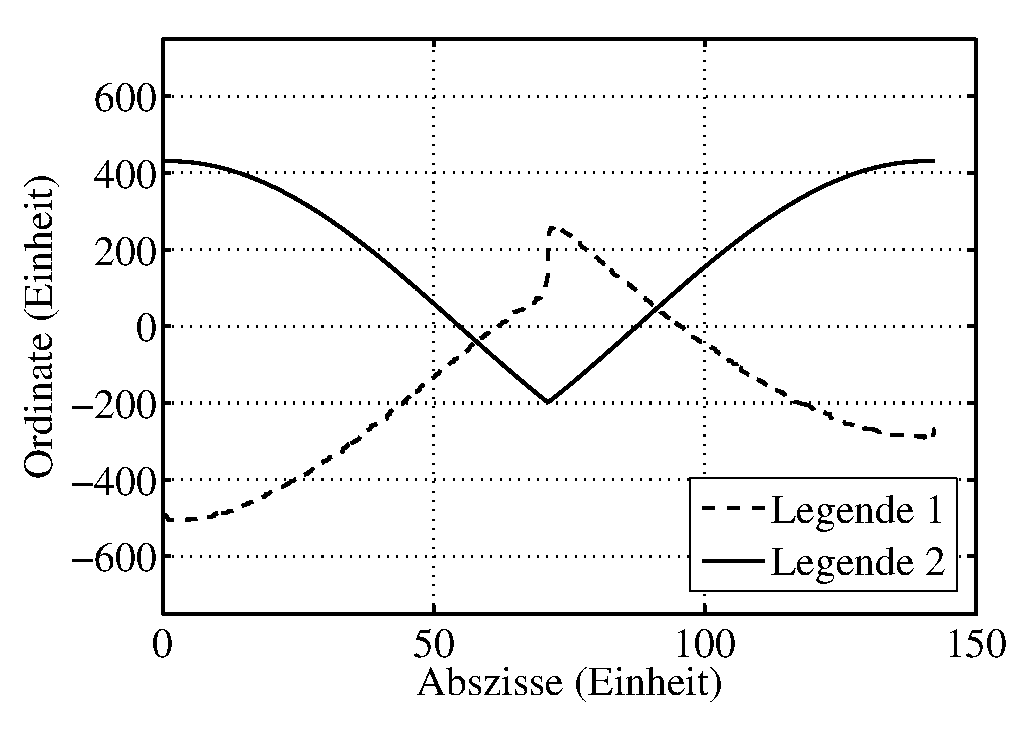
\includegraphics[width=9cm]{pic1}
  \caption{Musterdiagramm}
  \label{fig:pic1}
\end{figure}

Zudem muss bei nicht selbst erstellten Grafiken immer die Quelle
zitiert werden, dieses erfolgt in der Bildunterschrift.
(siehe Abbildung~\ref{fig:tud_logo}).

\begin{figure}[htbp]
  \centering
  
\includegraphics[width=6cm]{tud_logo_cmyk}
  \caption{Dargestellt ist das offizielle \cite{TuDo2}}
  \label{fig:tud_logo}
\end{figure}

\section{Hinweise zu Tabellen}
\label{hinweise:tabellen}

Tabellen enthalten ebenso wie Abbildungen eine fortlaufende
Nummerierung. Zudem ist jede Tabelle im Text zu erl�utern. Ihre
Schriftgr��e und Linienst�rke sind einheitlich so zu w�hlen, 
dass sie gut lesbar sind.

\begin{table}[htbp]
  \caption{Beispieltabelle}
  \renewcommand{\arraystretch}{1.3}
  \centering
  \begin{tabular}{cc}
	\toprule
    Konfiguration & Parametersatz \\
    \midrule
    $1$ & $\{p_{1}, \: p_{2}, \: p_{5}\}$ \\
    $2$ & $\{p_{1}, \: p_{4}, \: p_{5}\}$ \\
    $3$ & $\{p_{2}, \: p_{3}, \: p_{4}\}$ \\
    \bottomrule
    \end{tabular}
  \label{tab:bsp1}
\end{table}


\section{Hinweise zu Algorithmen}
\label{hinweise:algorithmen}

Dieser Abschnitt zeigt die Darstellungsweise von Algorithmen.
Algorithmus \ref{alg:pfadsuche} zeigt beispielsweise die Implementierung einer Tiefensuche zur Erkundung aller m�glichen Pfade zwischen einem Start- und Zielpunkt. 

\begin{algorithm}
  \caption{Suche alle m�glichen Pfade im HKP-Graphen}
    \label{alg:pfadsuche}
  \begin{algorithmic}[1]
    \Require{$G$: azyklischer Graph, $B$: Liste besuchter Knoten (Leer), $z$: Zielposition, $P$:~Liste aller Pfade (Leer)}
    \Statex
    \Function{suchePfade}{$G,B,z,P$}
      \Let{$b$}{$B$.back()} \Comment{Weise zuletzt besuchten Knoten zu}
      \For{jeden angrenzenden Knoten $v$ an Knoten $b$ in $G$}
       \If{$v \in B$} \Comment{Bereits besucht}
        \State \textbf{continue}
       \EndIf
       \If{$v$ == $z$} \Comment{Ziel erreicht}
        \State $B$.append($v$) \Comment{F�ge Ziel hinzu, um Pfad zu vervollst�ndigen}
        \State $P$.append($B$) \Comment{Speichere vollst�ndigen Pfad ab}
        \State \textbf{break}
       \EndIf
      \EndFor
      
      \For{jeden angrenzenden Knoten $v$ an Knoten $b$ in $G$}
       \If{$v \in B$ \textbf{or} $v$ == $z$} \Comment{Bereits besucht oder Ziel erreicht}
        \State \textbf{continue}        
       \EndIf
       \State $B$.append($v$) \Comment{\parbox[t]{0.6\columnwidth}{Dies ist ein Beispiel f�r einen sehr langen Kommentar im Pseudo-Code, der ohne diese Einstellung standardm��ig am Beginn der nachfolgenden Zeile weiter gef�hrt wird.}}
       \State \textsc{suchePfade}($G,B,z,P$) \Comment{Rekursionsschritt}
       \State $B$.pop($v$)
      \EndFor
    \EndFunction
  \end{algorithmic}
\end{algorithm}


\section{Hinweise zum Literaturverzeichnis}
\label{hinweise:literaturverzeichnis}

Das Literaturverzeichnis enth�lt alle relevanten Arbeiten und  die vollst�ndige Angabe aller
Quellen, die zur Bearbeitung des Themas herangezogen wurden. Dabei
sind diese an den entsprechenden Stellen im Text zu zitieren. \\

\textbf{Achtung}, der klassische Latex-Befehl \texttt{\textbackslash cite} ist nicht zu verwenden, da er mit dem vorgegebenen Biblatex-Paket nicht kompatibel ist! \\

Es wird im Allgemeinen wie folgt zitiert:

Im Text werden die Befehle 
\begin{verbatim}\textcite[Seitenangabe]{Bibtex-Key}\end{verbatim}
\begin{verbatim}\textcite{Bibtex-Key}\end{verbatim}
verwendet. Das hei�t, das Zitat ist als Teil des Satzes integriert.\\
Beispielsweise: \textcite[S. 123 ff.]{Book3} hat ein Verfahren entwickelt um ... 

Bei mehreren thematisch zusammengeh�renden Quellen werden die Bibtex-Keys durch Kommas separiert �bergeben.
\begin{verbatim}\textcite{Bibtex-Key1,Bibtex-Key2}\end{verbatim} 
Beispielsweise: \textcite{Book3, InProc4} befassen sich mit ...

Ohne konkrete Integration in den Text kann die Literaturquelle in Klammern angegeben werden. Dies erfolgt entsprechend �ber die Befehle 
\begin{verbatim}\parencite[Seitenangabe]{Bibtex-Key}\end{verbatim} 
und 
\begin{verbatim}\parencite{Bibtex-Key1,Bibtex-Key2}\end{verbatim} 
Beispielsweise: Entsprechende Verfahren sind aus der Literatur bekannt \parencite{Book3,InProc4}.

Ein Beispiel f�r den Aufbau eines resultierenden Literaturverzeichnisses finden Sie in dieser Vorlage.

\textbf{Achtung:} \textbf{Wikipedia} und ihre Inhalte unterliegen prinzipbedingt keiner wissenschaftlich anerkannten Qualit�tssicherung. Zudem sind die Inhalte dynamisch. Sie ist damit keine legitime wissenschaftliche Quelle und \textbf{sollte deshalb nicht als Quelle verwendet werden}. Wikipedia sollte \textbf{ausschlie�lich} als Anlaufstelle und Einstiegspunkt zum Auffinden geeigneter zitierf�higer wissenschaftlicher Quellen dienen, die in den \textbf{Einzelnachweisen} des jeweiligen Beitrags aufgelistet sind. 

Ist eine Verwendung aufgrund der Natur oder des Themas der Arbeit unvermeidlich bietet Wikipedia eine eigene \glqq Zitierhilfe\grqq, die entsprechende Bibtex-Eintr�ge erzeugt.

\section{Hinweise zum Anhang}
\label{hinweise:anhang}

Im Anhang k�nnen die Informationen, die in keinem direkten
Zusammenhang mit dem Inhalt einzelner Kapitel stehen f�r Ihre
Arbeit allerdings von Bedeutung sind (Pseudo-Code,
Komponentenbeschreibung, Kennfelder, etc.), dargestellt werden.

\section[Vorlage, Drucken und Binden]{Hinweise zur Vorlage, dem Drucken und Binden sowie einem Hinweis zu sehr langen Abschnittsnamen}
\label{hinweise:vorlage}

Diese Vorlage ist f�r einen beidseitigen Druck im DIN-A4-Format ausgelegt. In der gedruckten Version stehen die Seitenzahlen jeweils au�en in der Titelzeile. Auf der inneren Seite der Kopfzeile steht zur einfacheren Navigation auf der linken Seite Kapitelnummer und Kapitelname, rechts Nummer und Bezeichnung des aktuellen Abschnitts. Neue Kapitel starten jeweils auf der rechten Seite und haben die Seitennummer mittig in der Fu�zeile.
Sollte der Kapitel- oder Abschnittsname zu lang f�r die Kopfzeile oder Inhaltsverzeichnis sein sollte ein pr�gnanterer Name gefunden werden oder es wird ein Kurzname definiert, wie in diesem Abschnitt geschehen.

F�r das Binden der finalen Version der Arbeit erhalten Sie von ihrem Betreuer Deck- und R�ckseiten aus entsprechend bedrucktem farbigen Karton. Diese Seiten sind in dieser Vorlage nicht enthalten. Das Binden erfolgt durch eine (m�glichst schwarze) Klebebindung. Ein zus�tzlicher Einband (Klarsichtfolie oder Karton) ist nicht vorgesehen.\\

�nderungen an der \LaTeX-Vorlage sind in jedem Fall mit Ihrem Betreuer abzukl�ren!\\


\section{Hinweise zur Abgabe}
\label{hinweise:abgabe}

Der Absatz git f�r Studenten der Fakult�t Elektrotechnik und Informationstechnik der TU Dortmund. (Stand 2014).

Die Studentin/Der Student hat \textbf{drei gebundene Exemplare} sp�testens am Abgabetermin \textbf{im Dekanat einzureichen}. Bitte die Gesch�ftszeiten beachten! Zus�tzlich ist eine digitale Version abzugeben (CD oder DVD). Der Datentr�ger muss die Arbeit als PDF enthalten. Es d�rfen aber nat�rlich zus�tzliche Daten abgelegt werden.
% Daf�r muss ebenfalls das Formular &bdquo;Abgabebest�tigung&ldquo;, welches im Sekretariat des Lehrstuhls RST aufbewahrt wird, vom Studenten zum Quittieren der Abgabe dem Dekanat vorgelegt werden. 
Diese Belegexemplare werden an Professor Bertram weitergeleitet und sind die Grundlage der Bewertung.

Sie k�nnen selbst entscheiden, ob Sie die Arbeit in Farbe oder Schwarz-Wei� drucken wollen. Wir empfehlen aus Kostengr�nden den Schwarz-Wei�-Druck. Falls Lehrstuhl RST weitere Exemplare druckt, geschieht dies in Schwarz-Wei�, sodass in jedem Fall bei der Erstellung der Arbeit darauf zu achten ist, dass alle Abbildungen in Graustufen deutlich erkennbar sind.\\




%%%%%%%%%%%%%%%%%%%%%%%%%%%%%%%%%%%%%%%%%%%%







% #######################################################
% !TeX encoding = ISO-8859-1
\chapter[N�tzliche Latex-Informationen]{N�tzliche Latex-Informationen (Verwendung ist optional)}

\section{Latex-Distributionen und Editoren}

\LaTeX-Pakete und -Kompilierer haben den Vorteil, dass sie vollst�ndig unabh�ngig von dem sp�ter verwendeten Latex-Editor installiert werden k�nnen. Sie werden in sogenannten Latex-Distributionen zusammengefasst. Empfehlenswerte Distributionen sind unter Windows MikTeX (\href{http://miktex.org/}{http://miktex.org/}) und unter OS~X MacTeX \href{https://tug.org/mactex/}{https://tug.org/mactex/}.

Die Auswahl des Latex-Editors erfolgt in der Regel nach individuellen Bed�rfnissen und Geschmack.
Ein empfehlenswerter, plattform�bergreifender Editor ist TeXstudio \href{http://texstudio.sourceforge.net/}{http://texstudio.sourceforge.net/}. Dieser bietet unter anderem die M�glichkeit, gew�nschte Positionen der PDF-Vorschau unmittelbar im Quelltext anzuzeigen.
Ein weiterer verbreiteter Editor ist TeXnicCenter (\href{http://www.texniccenter.org/}{http://www.texniccenter.org/}).

Abschlie�end muss sich der Autor zwischen dem Latex- (PS/Dvi) und dem Pdflatex-Kompilierer entscheiden.
Die jeweilige Auswahl ist in den Einstellungen des verwendeten Editors zu treffen.\\

Pdflatex:
\begin{itemize}
	\item Fortschrittlicher als Latex
	\item Unterst�tzt folgende Bilddateitypen: PDF (Vektor), PNG, JPG.
	\item Unterst�tzt EPS-Bilder mit dem Paket "`epstopdf"' (bereits inkludiert).
	\item Nicht kompatibel mit alten Paketen, die nur mit PostScript-Dateien arbeiten.
\end{itemize}

Latex (PS/Dvi):
\begin{itemize}
	\item Funktioniert mit "`psfrag"' und anderen auf PS basierenden Paketen.
	\item Unterst�tzt ohne weitere Konvertierungen nur EPS-Bilder.
	\item L�ngere Kompilierungszeit
\end{itemize}


\section{Bild neben Tabelle}
Eine Tabelle neben einer Abbildung einf�gen unter Ber�cksichtigung der zugeh�rigen Verzeichnisse (Tabellen, Abbildungen):
\begin{figure}[htbp]
%
	\begin{minipage}[t]{0.45\textwidth}
	\centering
	\raisebox{2.5cm}{ %per hand
		\begin{tabular}{cc}
		\toprule
		Konfiguration & Parametersatz \\
		\midrule
		$1$ & $\{p_{1}, \: p_{2}, \: p_{5}\}$ \\
		$2$ & $\{p_{1}, \: p_{4}, \: p_{5}\}$ \\
		$3$ & $\{p_{2}, \: p_{3}, \: p_{4}\}$ \\
		\bottomrule
		\end{tabular}
	}
	\captionof{table}{Definitionsbereich der Parameter zur Optimierung.} %ins tabellenverzeichnis einf�gen
	\label{tab:bsp2}
	\end{minipage}
%
	\begin{minipage}[t]{0.45\textwidth}
	\centering
	  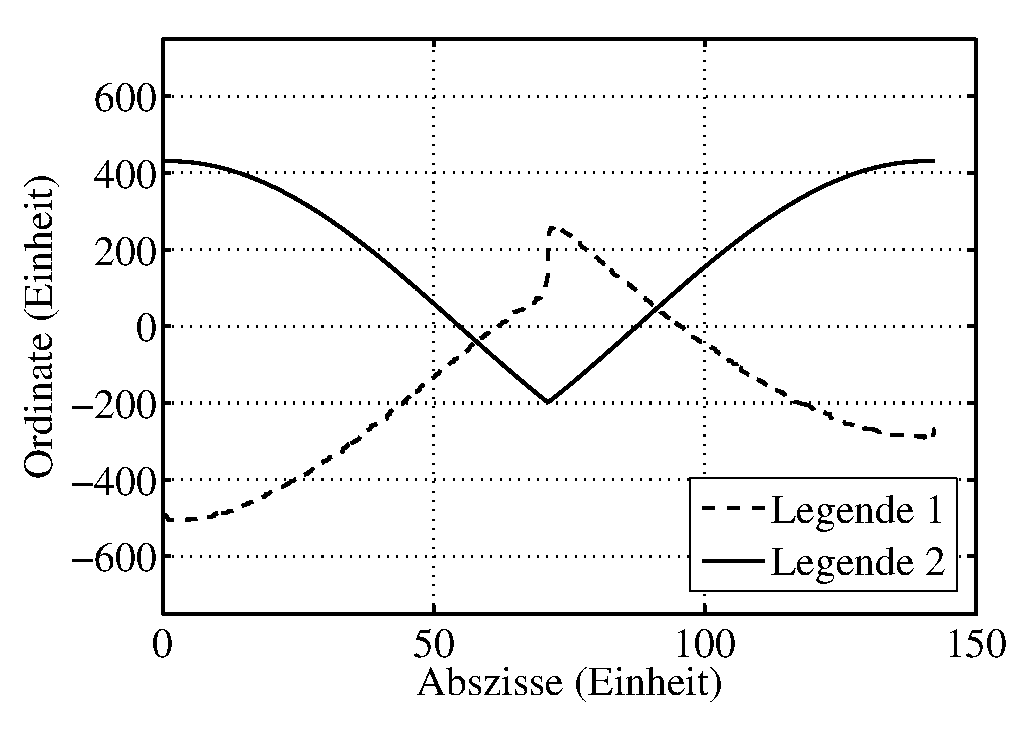
\includegraphics[width=\textwidth]{pic1}
  	\captionof{figure}{Musterdiagramm}
	\end{minipage}
\end{figure}


\section{Subcaption: Bild neben Bild und Tabelle neben Tabelle}

Das \textit{Subcaption} package (Beschriftung von Tabellen und Abbildungen mit a), b), ...) sollte ausschlie�lich gew�hlt werden,
wenn die zugeh�rigen Tabellen / Abbildungen auch wirklich kontextuell zusammengeh�ren.

\begin{figure}[htbp]
        \centering
        \begin{subfigure}[b]{0.3\textwidth}
        		\centering
                
\includegraphics[width=\textwidth]{tud_logo_rgb} 
                \caption{TU Dortmund Logo}
                \label{fig:subfigure_tud_logo}
        \end{subfigure}%
        \quad %add desired spacing between images, e. g. ~, \quad, \qquad, \hfill etc.
          %(or a blank line to force the subfigure onto a new line)
        \begin{subfigure}[b]{0.3\textwidth}
        		\centering
                
\includegraphics[width=0.3\textwidth]{rst_rgb} % relative width w.r.t. to the subfigure box
                \caption{RST Logo}
                \label{fig:subfigure_rst_rgb}
        \end{subfigure}
        \caption{Sammlung aller Logos}
        \label{fig:logos}
\end{figure}

F�r lange Beschreibungstexte kann die \textit{Subfigure-Caption} leer gelassen werden. Eine Beschreibung mit Referenz zu den Buchstaben a),..., erfolgt dann in der allgemeinen Beschreibung.

Tabelle \ref{tab:parameter_tabellen} listet alle verwendeten Parameter auf. Tabelle \ref{tab:parameter_tabelle1} ...

\begin{table}[htbp]
\caption{Hauptbeschriftung}
\centering
	\begin{subtable}[t]{.5\textwidth}
	\centering
			\caption{Tabelle links}
			\begin{tabular}{cc}
				\toprule
				Konfiguration & Parametersatz \\
				\midrule
				$1$ & $\{p_{1}, \: p_{2}, \: p_{5}\}$ \\
				$2$ & $\{p_{1}, \: p_{4}, \: p_{5}\}$ \\
				$3$ & $\{p_{2}, \: p_{3}, \: p_{4}\}$ \\
				\bottomrule
			\end{tabular}
			\label{tab:parameter_tabelle1}
	\end{subtable}%
	\begin{subtable}[t]{.5\textwidth}
			\centering
			\caption{Tabelle rechts}
			\begin{tabular}{cc}
				\toprule
				Konfiguration & Parametersatz \\
				\midrule
				$1$ & $\{p_{1}, \: p_{2}, \: p_{5}\}$ \\
				$2$ & $\{p_{1}, \: p_{4}, \: p_{5}\}$ \\
				$3$ & $\{p_{2}, \: p_{3}, \: p_{4}\}$ \\
				\bottomrule
			\end{tabular}
			\label{tab:parameter_tabelle2}
	\end{subtable}
	\label{tab:parameter_tabellen}
\end{table}




%
%
%
%%%%%%%%%%%%%%%%%%%%%%%%%%%%%%%%%%%%%%%%%%%%
\newpage
\section{eps-Tagging mit psfrag}
\textit{Achtung: eps-Tagging funktioniert nur mit "`latex ps/dvi"' und nicht mit "`pdflatex"'.\\
Alternativ siehe tikz im Zusammenhang mit Matlab-Plots in Abschnitt \ref{sec:tikz}.}\\

Mit Hilfe des Packets psfrag kann die Beschriftung von Abbildungen unabh�ngig von der eigentlichen Grafik erfolgen.\\
Im Klartext:
\begin{itemize}
  \item Schriftart direkt aus Latex �nderbar (z.\,B. identische Schrifart wie �briger Text)
  \item Schriftgr��e direkt aus Latex �nderbar (wird daher unabh�ngig von der Skalierung der Abbildung dargestellt)
  \item Gewohnte Latex-Syntax anwendbar (Formel, Tabellen, etc.)
\end{itemize}
N�heres in der Doku zu lesen unter:\\
\emph{http://www.ctan.org/tex-archive/help/Catalogue/entries/psfrag.html}.
Soll ein Graph o.\,�. aus Matlab in das Dokument eingef�gt werden, so kann das Exportieren in eps inklusive Tagging automatisch geschehen:\\ \emph{http://www.mathworks.com/matlabcentral/fileexchange/21286-matlabfrag}\\
%
%
\begin{figure}[H]%
\centering
	\begin{subfigure}[t]{0.45\linewidth} %t for top alignment, b for bottom alignment
		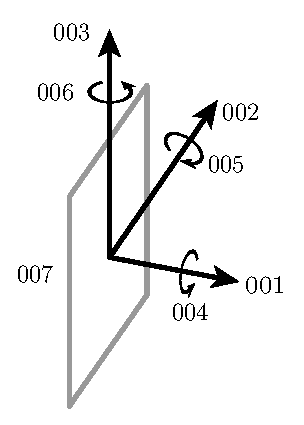
\includegraphics[width=\textwidth]{ref-CS}	
		\caption{Bild mit Tags}
		\label{fig:refCs}
	\end{subfigure}
	\quad %add desired spacing between images, e. g. ~, \quad, \qquad, \hfill etc.
	  %(or a blank line to force the subfigure onto a new line)
	\begin{subfigure}[t]{0.45\linewidth} 
		\psfrag{001}[lc][lc]{ \small \textbf{x}}%  % WORKS ONLY WITH LATEX AND NOT WITH PDFLATEX
		\psfrag{002}[lc][lc]{ \small \textbf{y}}%
		\psfrag{003}[lc][lc]{ \small \textbf{z}}%
		\psfrag{004}[tc][tc]{ \small ${\gamma}$}%
		\psfrag{005}[lc][lc]{ \small ${\beta}$}%
		\psfrag{006}[rc][rc][1][45]{ \small ${\alpha}$}%
		\psfrag{007}[rc][rc]{}%Tag aus dem Bild entfernen
		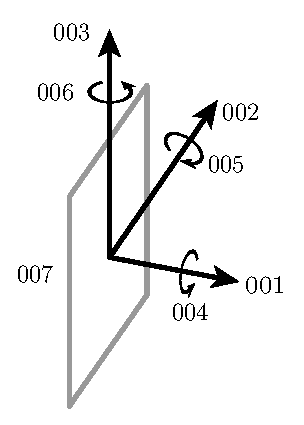
\includegraphics[width=\textwidth]{ref-CS}	
		\caption{Bild mit ersetzten Tags (Nur falls mit DVI-PS Latex kompiliert)}
		\label{fig:refCs2}
	\end{subfigure}
\caption[Eintrags ins Abb-VZ]{Abbildung mit 2 Subfigures und psfrag-Tagging.}
\end{figure}





\clearpage
\section{Zeichnungen und Matlab-Plots mit Tikz}
\label{sec:tikz}

Tikz ist ein umfangreiches \LaTeX-Paket, mit dem Bilder �ber Programmanweisungen erstellt werden k�nnen.
Zahlreiche Anleitungen und Beispiele k�nnen unter dem folgenden Link eingesehen werden:\\ 
\href{http://www.texample.net/tikz/examples/}{\emph{http://www.texample.net/tikz/examples/}}
\\

Eine besonders n�tzliche Anwendung entsteht aus der Kombination mit dem Matlab-Plugin "`matlab2tikz"':\\
\href{http://www.mathworks.com/matlabcentral/fileexchange/22022-matlab2tikz}{\emph{http://www.mathworks.com/matlabcentral/fileexchange/22022-matlab2tikz}}\\
Hiermit k�nnen in Matlab erstellte Bilder in ein Tikz-Bild umgewandelt werden. Ein Vorteil ist die einfache M�glichkeit, anschlie�end beliebige Attribute des Bildes beziehungsweise der Zeichnung anzupassen: Linienfarbe, -breite, -typ, Gitter, Legenden, Marker, u.a.

Die prinzipielle Vorgehensweise ist wie folgt:
\begin{enumerate}
	\item Matlab Zeichnung erstellen und in den Vordergrund holen (am Besten alle anderen Bilder schlie�en).
		Attribute der Zeichnung k�nnen auch schon hier angepasst werden (Gitter, Linienfarbe, -breite, Log-Skalierung,...).
	\item Nachdem "`matlab2tikz"' in den Matlab-Pfaden hinzugef�gt wurde, kann das Bild konvertiert werden:\\
		\textit{matlab2tikz('myfile.tikz', 'height', '\textbackslash figureheight', 'width', '\textbackslash figurewidth');} \\
		Die Variablen \textbackslash figureheight und \textbackslash figurewidth erlauben die sp�tere beliebige Anpassung der Gr��e des Bildes.
	\item \textit{myfile.tikz} in das Abbildungsverzeichnis dieser Arbeit kopieren.
	\item Tikz-Bild nach dem unten aufgef�hrten Beispiel einbinden (siehe Quellcode).
	\item \textit{myfile.tikz} beliebig ver�ndern. Google hilft bei vielen speziellen W�nschen. 
\end{enumerate}


\begin{figure}[h]
\centering
%\tikzexternaldisable
\includetikz[0.9\textwidth][5cm]{x_square} %[width][height][filename without ./Abbildungen/...)]
\caption{Quadratische Funktion}
\label{fig:tikz:x_square}
\end{figure}


\subsection{Tikz externalisieren}

Wer viele Tikz-Bilder einbindet oder Tikz-Bilder mit einer sehr gro�en Anzahl an Datenpunkten verwendet, der wird zwangsl�ufig 
auf lange Kompilierungszeiten beziehungsweise Abbr�che aufgrund eines �berf�llten Latex-Zwischenspeichers sto�en.

Um dieses Problem zu vermeiden und die Kompilierungszeit erheblich zu erh�hen, bietet Tikz die M�glichkeit, Bilder vorzukompilieren. Damit werden vollautomatisiert eps/pdf Bilder aus dem Tikz-Quelltext erzeugt und anschlie�end intern eingebunden.
Die notwendigen Konfigurationen sind in "`packages.tex"' bereits voreingestellt. Die einzige, benutzerseitige �nderung erfolgt im verwendeten Latexeditor. Dem Latex- beziehungsweise PdfLatex-Kompilierer muss die Erlaubnis erteilt werden,
Shell-Scripte auszuf�hren.
Dazu die Argumentliste in den Editor-Einstellungen um folgenden kompilierer- und systemspezifischen Eintrag erweitern:\\

Bei Windows-Systemen (MikTeX):
\begin{itemize}
	\item	\textit{latex.exe [other arguments] -enable-write18 \%.tex}
 	\item 	\textit{ pdflatex.exe [other arguments] -enable-write18 \%.tex}
\end{itemize}

Bei Unix-Systemen (MacTeX/Linux):
\begin{itemize}
	\item	\textit{latex.exe [other arguments] -shell-escape \%.tex}
	\item 	\textit{pdflatex.exe [other arguments] -shell-escape \%.tex}
\end{itemize}

\vspace{\baselineskip}
Im Folgenden werden einige zu beachtende Hinweise zur Vorkompilierung aufgelistet:
\begin{itemize}
	\item Bitte das Paket "`pgfplots"' stets auf die neuste Version aktualisieren (z.B. mit dem Miktex Update-Manager), da hier noch viele Fehlerbehebungen u.a. durchgef�hrt werden.
	\item Der Ordner "`./Abbildungen/tikz-extern"' muss vorhanden sein.
	\item Neuere Latex-Distributionen (>2013) erkennen �ber den Vergleich der Pr�fsummen, ob das Tikz-Bild ge�ndert worden ist und f�hren demnach ein erneutes Kompilieren des Tikz-Bildes automatisch aus.
	\item Werden Standardwerte von Tikz au�erhalb der "`*.tikz"' Datei ver�ndert, erfolgt keine automatische Neukompilierung, da die Pr�fsummen unver�ndert sind.
	Der Befehl\texttt{ \textbackslash tikzset\{external/force remake\}} kann im Dokumentenkopf gesetzt werden, um eine Neukompilierung aller Tikz-Bilder zu erzwingen.\\
	Der Befehl\texttt{ \textbackslash tikzset\{external/force remake next\}} kann vor das jeweilige Bild gesetzt werden, um eine Neukompilierung des nachfolgenden Tikz-Bildes zu erzwingen (Latex Distributionen >2013).\\
	\texttt{\textbackslash tikzexternaldisable} am Anfang der jeweiligen "`Figure"'-Umgebung einf�gen, falls das Bild generell von der Externalisierung ausgeschlossen werden soll.\\
	Alternativ k�nnen tempor�re Dateien gel�scht werden.
	\item Sollte es trotz der Externalisierung zu �berl�ufen des Latex-Puffers kommen, gibt es zwei m�gliche Ursachen.
	\begin{enumerate}
		\item Das "`Externalisieren"' wurde nicht erfolgreich aktiviert. Bitte f�hren Sie die o.g. Schritte durch, l�schen die tempor�ren, "`vorkompilierten"' Vektorbilddateien, und kompilieren dieses Thesis-Beispielmuster inklusive dem Test-Bild (siehe Abbildung \ref{fig:tikz:x_square}) erneut. Pr�fen Sie, ob "`./Abbildungen/tikz-extern/x\_square.pdf"' (pdflatex) bzw. "`x\_square.ps"' (ps/dvi) vorhanden und lesbar ist.
		\item Falls in einem Bild so viele Datenpunkte vorhanden sind, dass der Latex-Puffer selbst beim kompilieren dieses einen Bildes �berl�uft, hilft die Externalisierung auch nicht weiter (tritt bei gro�en \textit{mesh-} und \textit{surface-plots} �fter mal auf). In diesem Fall entweder das Bild komprimieren, oder ohne die Verwendung von Tikz exportieren (bspw. mit direktem eps/pdf-Export in Matlab).
		Eine weitere unsaubere L�sung ist, den Latex-Puffer auf dem lokalen Rechner zu erh�hen, um somit das berechnete Vektorbild zu erhalten. Hier kann nachtr�glich auch der Tikz-Code durch eine gew�hnliche Bildeinbindung mit dem zuvor generierten pdf ersetzt werden.
	\end{enumerate}
	
\end{itemize}




\subsection{Zeichnen mit Tikz}

Tikz kann auch f�r Blockschaltbilder u.a. verwendet werden (siehe oben verlinkte Sammlung an Beispielen).
Anleitungen findet man bei Google wie Sand am Meer.

\externalizeOff
\begin{figure}[htb]
	\centering
	\begin{tikzpicture}[->,>=stealth',shorten >=1pt,auto,node distance=3cm, thick]
	 		\tikzstyle{main node}=[circle,fill=black!40,draw,font=\sffamily\Large\bfseries]
	 		\node[main node] (1) {1};
	 		\node[main node] (2) [below left of=1] {2};
	 		\node[main node] (3) [below right of=2] {3};
	 		\node[main node] (4) [below right of=1] {4};
	 		
	 		\path[every node/.style={font=\sffamily\small}]
	 		(1) edge node [left] {0.6} (4)
	 		edge [bend right] node[left] {0.3} (2)
	 		edge [loop above] node {0.1} (1)
	 		(2) edge node [right] {0.4} (1)
	 		edge node {0.3} (4)
	 		edge [loop left] node {0.4} (2)
	 		edge [bend right] node[left] {0.1} (3)
	 		(3) edge node [right] {0.8} (2)
	 		edge [bend right] node[right] {0.2} (4)
	 		(4) edge node [left] {0.2} (3)
	 		edge [loop right] node {0.6} (4)
	 		edge [bend right] node[right] {0.2} (1);
	\end{tikzpicture}
	\caption{Gezeichnet mit Tikz}
\end{figure}
\externalizeOn

\externalizeOff
\begin{figure}[htb]
	\centering
	\begin{tikzpicture}[align=center,auto]
		% Tikz example adapted from http://www.texample.net/tikz/examples/tag/block-diagrams/
		% Elemente
		\tikzstyle{block} = [draw, rectangle, minimum height=1em, minimum width=2em]
		\tikzstyle{sum} = [draw, circle]
		%\tikzstyle{every node}=[font=\tiny] % set fontsize for all nodes
		
		% Bl�cke:
		\node[coordinate] (input) {};
		\node[sum] (sum) [right=0.6cm of input] {};
		\node[block] (controller) [right=0.7cm of sum] {Controller};
		\node[block] (system) [right=0.7cm of controller] {System};
		\node[coordinate] (output) [right=0.8cm of system] {};
		
		% Verbindungen
		\draw [->] (controller) -- node[name=u] {$u$} (system);
		\draw [draw,->] (input) -- node {$w$} (sum);
		\draw [->] (sum) -- node {$e$} (controller);
		\draw [->] (system) -- node [name=y] {$y$}(output);
		\draw [->] (y) |- ([yshift=-1.5em]system.south) -| node[pos=0.99] {$-$} node [near end] {$y_m$} (sum); %
	\end{tikzpicture}
	\caption{Blockschaltbild mit Tikz}
\end{figure}
\externalizeOn




\externalizeOff
\begin{figure}[htb]
	\centering	
	\begin{tikzpicture}%[trim axis left]
		\begin{axis}[
		  width = 0.9\textwidth,
		  height = 6cm,
		  domain = 0.001:10,
		  samples = 100,
		  grid = both,
		  xlabel = $\delta$,
		  ylabel = Weights,
		  legend pos = south east] % customize the axis environment with whatever you want (xmax,ymin,...)	  
		\addplot [color=black, solid, line width=1.5pt] {0.5*tanh(x-3)+0.5}; \addlegendentry{$\sigma$};
		\addplot [color=gray, dashed, line width=1.5pt] {1-(0.5*tanh(x-3)+0.5)}; \addlegendentry{$(1-\sigma)$};
		\end{axis}
	\end{tikzpicture}
	\caption{Plot mit Tikz (ohne Umweg �ber Matlab)}
\end{figure}
\externalizeOn




\externalizeOff
\begin{figure}[htb]
	% Define block styles
	\tikzstyle{decision} = [diamond, draw, %fill=green!20, 
		text width=4.0em, text badly centered, node distance=2cm, inner sep=0pt]
	\tikzstyle{block} = [rectangle, draw, %fill=green!20, 
	text width=5em, text centered, rounded corners, minimum height=2em]
	\tikzstyle{line} = [draw, -latex']
	\tikzstyle{cloud} = [draw, ellipse, %fill=orange!40,
				 node distance=3cm, minimum height=2em]
	
	\begin{center}
		\begin{tikzpicture}[node distance = 1.4cm, auto, every node/.style={font=\sffamily\scriptsize}]
		% Place nodes
		\node [block] (init) {initialize model};
		\node [cloud, left of=init] (expert) {expert};
		\node [cloud, right of=init] (system) {system};
		\node [block, below of=init] (identify) {identify candidate models};
		\node [block, below of=identify] (evaluate) {evaluate candidate models};
		\node [block, left of=evaluate, node distance=3cm] (update) {update model};
		\node [decision, below of=evaluate] (decide) {is best candidate better?};
		\node [block, below of=decide, node distance=1.9cm] (stop) {stop};
		% Draw edges
		\path [line] (init) -- (identify);
		\path [line] (identify) -- (evaluate);
		\path [line] (evaluate) -- (decide);
		\path [line] (decide) -| node [near start] {yes} (update);
		\path [line] (update) |- (identify);
		\path [line] (decide) -- node {no}(stop);
		\path [line,dashed] (expert) -- (init);
		\path [line,dashed] (system) -- (init);
		\path [line,dashed] (system) |- (evaluate);
		\end{tikzpicture}
	\end{center}
	\caption{Ablaufdiagramm mit Tikz}
\end{figure}
\externalizeOn
%
%
%



% #######################################################
% !TeX encoding = ISO-8859-1
%%%%%%%%%%%%%%%%%%%%%%%%%%%%%%%%%%%%%%%%%%%%%%%%%%%%%%%%%%%%
\chapter{Linkliste f�r n�tzliche Tools rundum Latex und Grafiken}
Latex
\begin{compactitem}
	\item \emph{http://miktex.org/}   \\ Windows Latex Distribution
	\item \emph{https://tug.org/mactex/}   \\ Os~X Latex Distribution
	\item \emph{http://texstudio.sourceforge.net/}  \\ TeXstudio Entwicklungsumgebung (empfohlen)
	\item \emph{http://www.texniccenter.org/}  \\ TeXnicCenter Entwicklungsumgebung
	\item \emph{http://de.wikipedia.org/wiki/Hilfe:TeX}   \\ Sammlung mathematischer Befehle
	\item \emph{http://www.ctan.org/} \\ Dokus aller Pakete
	\item \emph{http://en.wikibooks.org/wiki/LaTeX/} \\ HILFE
	\item \emph{http://www.texify.com/}	\\ Latex Code per Copy/Paste ausprobieren (Formeln)
\end{compactitem}
Grafiken
\begin{compactitem}
	\item \emph{http://www.inkscape.org/}   \\ Vektorgrafiken
	\item \emph{http://www.imagemagick.org/}  \\ konvertierten von *.* nach eps	
\end{compactitem}
Matlab
\begin{compactitem}
	\item \emph{http://www.mathworks.com/matlabcentral/fileexchange/22022-matlab2tikz} \\ exportiert figure nach tikz
	\item \emph{http://www.mathworks.com/matlabcentral/fileexchange/21286-matlabfrag} \\ exportiert figure nach eps + tags
	\item \emph{http://www.mathworks.com/matlabcentral/fileexchange/23604-fixlines} \\ ersetzt ''Matlab''-Linien mit ''vern�nftigen'' Linien
	\item \emph{http://www.mathworks.com/matlabcentral/fileexchange/23629-exportfig} \\ exportiert figure nach eps, pdf, etc. (mit fixlines, ohne tagging)
\end{compactitem}


% ##########################################################################
% BIBLIOGRAPHY
% ##########################################################################

\printbibliography

% ##########################################################################
% APPENDIX
% ##########################################################################
\appendix

% !TeX encoding = ISO-8859-1
\chapter{\iftoggle{lang_eng}{Appendix}{Anhang}}
\label{app:Anhang1}
Das ist der Anhang (optional).



% ##########################################################################
% THAT'S IT!
% ##########################################################################
\end{document}